\documentclass[10pt]{article}
\usepackage[a4paper,margin=2cm]{geometry}
\usepackage{booktabs,longtable,amsmath,amssymb,graphicx,pdfpages,caption,lscape}
\captionsetup{font=small,labelfont=bf}
\title{\bfseries Multi-region CL inflow fits of the SPARC category-D galaxies:\\ can the structured residuals be absorbed by the existing model extensions?}
\author{Automated analysis for E.P.J.\ de Haas}\date{}
\begin{document}\maketitle
\section*{Summary}
Category D contains the 18 SPARC galaxies whose single-Lagrangian (single-L) residuals are significantly structured (runs test $p<0.05$) but match neither the $+-+$ template of category B nor the $-+-$ template of category C. Before attributing their kinematics to the history of the galaxy (mergers, accretion), we test whether the existing CL model extensions absorb the structure: one virial window [1,2], two Lagrangians [2], two virial windows [1], and two Lagrangians with a disk window. The result is a split into four groups, not a single class. (i) In 6 galaxies no extension is justified ($\Delta\mathrm{BIC}\ge-6$): the sign pattern is real, but its amplitude lies within the SPARC errors (single-L $\chi^2_\nu=0.03$--$0.26$). (ii) 3 galaxies are described cleanly by one of the extensions with well-determined parameters. (iii) 4 are improved, but their parameters are poorly constrained. (iv) 5 bulge-dominated S0--Sbc galaxies are improved enormously ($\Delta\mathrm{BIC}$ down to $-3916$), but only with unphysical parameters: the inner CL bulge collapses ($R\to0$) and window strengths reach $|p|>100$. For this group the structure points to a missing bulge component rather than to history. Category D therefore does not support the general conclusion that historical dynamics dominate. It is mainly a mixture of residuals within the errors, curves needing more regions, and massive bulges not represented by the CL bulge.

\section{Models}
All models use the CL inflow quantities $X=\sqrt{2GM/R}-H_zR$ and $Y(r)=\sqrt{2GM/r}-H_zr$ with $H_z=2.2\times10^{-18}\,\mathrm{s^{-1}}$ and are fitted to $v^2$ with $\sigma_{v^2}=2V_\mathrm{obs}\delta V_\mathrm{obs}$.
\begin{itemize}\itemsep1pt
\item \textbf{S} single-L [2, Eqs.~17--18]: $v^2=\tfrac12X^2r^2/R^2$ ($r\le R$), $\tfrac32X^2-Y^2$ ($r>R$); $k=2$.
\item \textbf{VW} one virial window [1, Eq.~6; 2, Eq.~19]: $+\,p[\tfrac12Y(r)^2-\Phi_p]$ for $r\ge r_v$; $k=4$.
\item \textbf{2L} two Lagrangians [2, Eqs.~24--26]: $L_1(M_1,R_1)$ up to $R_2$, $L_2(M_2,R_2)$ beyond; $k=4$.
\item \textbf{VW2} two virial windows [1, Eqs.~5--7]: strength $p$ on $[r_{v1},r_{v2})$, $q$ beyond $r_{v2}$; $k=6$.
\item \textbf{2LVW} two Lagrangians with a window of strength $p$ in the $L_2$ disk beyond $r_v>R_2$; $k=6$.
\end{itemize}
Window gauges $\Phi$ are fixed by continuity of $v^2$ at each window radius, and window strengths are fitted as descent masses $M_N=(p-2)M$ (see the category-C report). For $H_z\to0$ a window adds $GM_N/r$ plus a constant, so $p>2$ is a Keplerian descent, $0<p<2$ a flattening and $p<0$ an extra rise.

\paragraph{Selection.} The preferred model has the lowest BIC, with a simpler model preferred when it lies within $\Delta\mathrm{BIC}<2$. An extension is accepted only if it beats single-L by $\Delta\mathrm{BIC}<-6$. For galaxies with $n\le7$ the six-parameter models are not fitted.
\paragraph{Status of the preferred fit.} \textbf{Clean}: all parameters within 60\%, no parameter at a bound, $|p|,|q|\le100$, $\chi^2_\nu\le2$. \textbf{Weakly constrained}: some parameter uncertainty above 60\% (degenerate radii or masses), or $\chi^2_\nu>2$. \textbf{Phenomenological}: the bulge radius at its lower bound ($R\le0.025$\,kpc) or a window strength $|p|>100$; the fit is statistically excellent but the parameters have no physical CL reading. Uncertainties: covariance, leave-one-out jackknife, distance/inclination refits and an $H_z=0$ refit, as in the A--C reports.

\section{Outcome}
\begin{table}[h]\centering\small\caption{Category-D outcome by status of the preferred fit.}\begin{tabular}{llp{9.5cm}}\toprule Status & $N$ & Galaxies (type, preferred model)\\\midrule
single-L adequate & 6 & DDO064 (Im, single-L), F563--1 (Sm, single-L), NGC0024 (Sc, single-L), NGC2915 (BCD, single-L), PGC51017 (BCD, single-L), UGC01281 (Sdm, single-L)\\
clean & 3 & NGC0300 (Sd, one window), NGC2841 (Sb, two windows), NGC6015 (Scd, two-L + disk window)\\
weakly constrained & 4 & NGC1090 (Sbc, two-L + disk window), NGC4138 (S0, one window), NGC7814 (Sab, one window), UGC00128 (Sdm, two windows)\\
phenomenological & 5 & NGC0289 (Sbc, two windows), UGC02487 (S0, two windows), UGC03546 (Sa, two windows), UGC06786 (S0, two windows), UGC09133 (Sab, two windows)\\
\bottomrule\end{tabular}\end{table}
\begin{figure}[h]\centering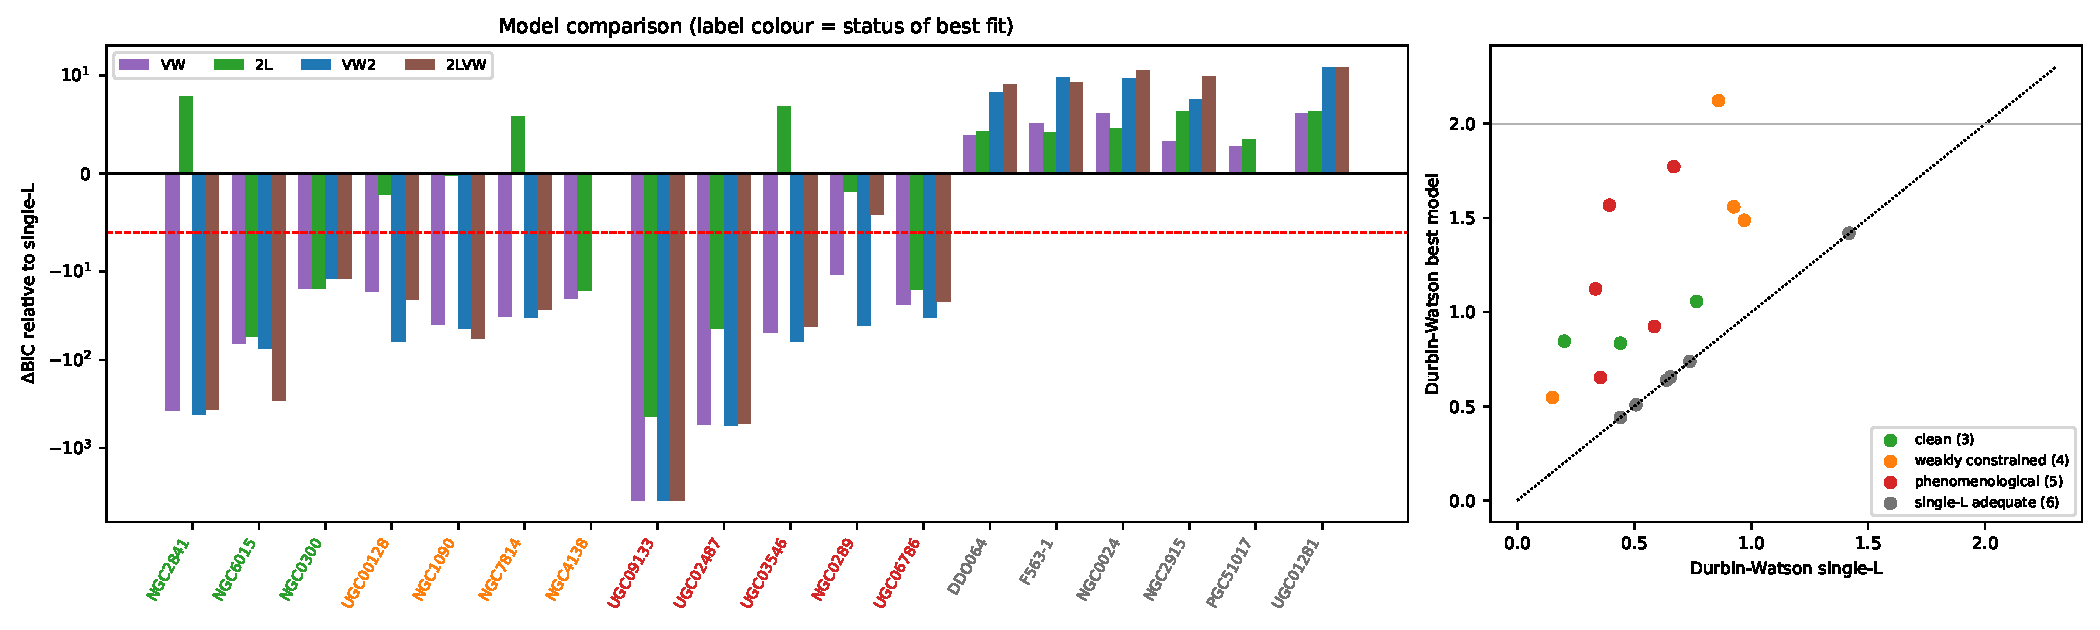
\includegraphics[width=\textwidth]{catD_fig_models.pdf}\caption{Left: $\Delta$BIC of each extension relative to single-L (symlog scale; red: $-6$). Galaxy labels are coloured by the status of the preferred fit: clean (green), weakly constrained (orange), phenomenological (red), single-L adequate (grey). Right: Durbin--Watson statistic, single-L versus preferred model.}\end{figure}
\paragraph{Single-L adequate (6).} DDO064, F563--1, NGC0024, NGC2915, PGC51017, UGC01281. These are mostly late types and dwarfs (Im, Sm, Sc, BCD, BCD, Sdm) with very small single-L $\chi^2_\nu$ (median 0.24). The runs test detects a coherent sign pattern, but no extension improves BIC, because the pattern lies well inside the error bars. UGC 1281 ($\chi^2_\nu=0.03$) is the galaxy for which [1] introduced the virial term on the basis of its outer six points. With the full error bars and BIC this refinement is not statistically required; [1] reported the same, a reduction of RMS$_\mathrm{rel}$ from 6.5\% to 6.3\%.

\paragraph{Clean (3).} NGC 2841 (Sb) is described by two windows: a Keplerian descent ($p\approx14$) beyond $r_{v1}\approx13$\,kpc, followed by a renewed rise ($q<0$) beyond $r_{v2}\approx44$\,kpc. $\chi^2_\nu$ falls from 9.3 to 0.40 and $\Delta\mathrm{BIC}=-413$. This is a category-C descent with an outer rise, exactly the two-window configuration of [1]. NGC 6015 (Scd) is described by a Lagrangian reset at $R_2\approx2.3$\,kpc followed by a flattening window ($p\approx1.8$) at $r_v\approx3.5$\,kpc, i.e.\ a B-type and a C-type feature combined ($\chi^2_\nu$ 8.7$\to$1.7). NGC 300 (Sd) needs one rising window ($p<0$) at $r_v\approx2.5$\,kpc. Two-L is equally good here ($\Delta\mathrm{BIC}$ +0.05), so NGC 300 is a B/C borderline case.

\paragraph{Weakly constrained (4).} NGC 7814 (Sab) is a descent from the first point; the window reproduces it ($\chi^2_\nu$ 2.96$\to$0.67), but $R$ and $r_v$ (0.4 and 0.9\,kpc) are degenerate with the inner masses. NGC 4138 (S0) has only 7 points. NGC 1090 (Sbc) prefers a two-L + window fit in which $R_2$ collapses onto $R_1$, i.e.\ effectively one window with a mass change. UGC 128 (Sdm) is improved by two windows ($\chi^2_\nu$ 6.1$\to$2.9) but remains structured. These galaxies are compatible with the C or B pictures, but the data do not fix the parameters.

\paragraph{Phenomenological (5).} NGC0289, UGC02487, UGC03546, UGC06786, UGC09133 (Sbc, S0, Sa, S0, Sab). Two virial windows lower $\chi^2_\nu$ dramatically (UGC 9133: 64$\to$4.7; UGC 2487: 38$\to$0.66), but in every case the parameters become extreme: the inner CL bulge shrinks to $R\le0.06$\,kpc (four of five) and window strengths reach $|p|$ or $|q|\approx10^2$--$3\times10^3$. The windows then act as a flexible spline, not as virial regions. All five are early and intermediate types (S0--Sbc) with prominent bulges: they have a sharp inner peak that the parabolic CL bulge ($v^2\propto r^2$ inside $R$) cannot follow. The structure in their residuals is therefore a model limitation of the bulge description and should not be read as evidence of history.
\section{Fit quality of the accepted extensions}
\begin{table}[h]\centering\small\caption{Fit-quality statistics (medians, single-L $\to$ preferred model).}\begin{tabular}{lrrr}\toprule & Clean (3) & Weakly constrained (4) & Phenomenological (5)\\\midrule
$\chi^2_\nu$ & 8.66 $\to$ 0.40 & 4.27 $\to$ 0.60 & 3.40 $\to$ 0.73\\
RMS$_\mathrm{rel}$ & 0.140 $\to$ 0.064 & 0.154 $\to$ 0.075 & 0.175 $\to$ 0.035\\
Durbin--Watson & 0.44 $\to$ 0.85 & 0.89 $\to$ 1.52 & 0.39 $\to$ 1.12\\
$p_\mathrm{runs}<0.05$ after & 3/3 & 1/4 & 4/5\\
$\Delta$BIC (median) & -286 & -45 & -63\\
\bottomrule\end{tabular}\end{table}
Residual structure remains (runs $p<0.05$) in 8 of the 12 accepted fits, including NGC 2841 and NGC 6015. These are high-precision curves (Q=1--2, $n=44$--50) in which small coherent deviations, e.g.\ from spiral-arm streaming, become significant at the few-per-cent level (RMS$_\mathrm{rel}$ 0.02--0.06). As in categories A--C, the SPARC errors are conservative for most galaxies. Distance and inclination systematics are of the same order as the statistical errors. Setting $H_z=0$ changes the clean fits by at most 7\%; the phenomenological fits move by up to about 110\%, consistent with their degeneracy.
\section{Assessment: history versus model structure}
\textbf{Can the dynamics of category D be attributed to the history of the galaxies?} Not on the basis of these fits. Step 1 shows that the class is heterogeneous:
\begin{enumerate}\itemsep1pt
\item \textbf{6 galaxies} have structure within the errors; single-L is statistically sufficient.
\item \textbf{7 galaxies} are absorbed, cleanly or with weak constraints, by the existing extensions of [1,2]: descent and rising windows, a Lagrangian reset, or combinations of these. They are B- and C-type features that occur together or close to the centre, which is why the single-template classification missed them.
\item \textbf{5 bulge-dominated S0--Sbc galaxies} require unphysical parameters. Their residuals trace a massive, compact bulge that the CL bulge parabola cannot represent, which is a limitation of the inner model.
\end{enumerate}
Galaxy history (accretion, mergers, settled virial matter) remains the interpretation proposed in [1] for virial windows in general. That applies equally to categories C and D, and is not established for D specifically. A history-specific conclusion would require step 2: comparing the galaxies that still need windows with independent indicators of disturbance, such as lopsided or tidal morphology, approaching/receding asymmetry of the rotation curve, HI warps and environment. For the phenomenological group, a separate bulge component is needed first: either a Newtonian or CL bulge with its own scale, or the inner bulge region of [1] with a free inner profile. Only then can its residual structure be interpreted.

\section*{References}\small
[1] E.P.J.\ de Haas (2026), From Rotation Curves to Cosmic Time: Probing High-Redshift Expansion through Nested Spiral Dynamics, \emph{J.\ High Energy Phys.\ Grav.\ Cosmol.} 12, 334--367, doi:10.4236/jhepgc.2026.121022 (virial term Eq.~3; multi-region virial model Eqs.~5--7).\par
[2] E.P.J.\ de Haas, Galactic Rotation Curves and the Constant--Lagrangian Field: Empirical Tests within the $Q_g$ Rotor Framework (manuscript; single-L Eqs.~17--18, virial term Eq.~19, two-L Eqs.~24--26).\par
[3] F.\ Lelli, S.S.\ McGaugh, J.M.\ Schombert (2016), SPARC, \emph{AJ} 152, 157.

\clearpage\begin{landscape}{\scriptsize\setlength{\tabcolsep}{3pt}
\begin{longtable}{lllrlrrrrrrrrll}
\caption{All category-D galaxies: residual signs of the single-L fit and model comparison ($\Delta$BIC relative to single-L; -- = not fitted, $n\le7$).}\\\toprule
Galaxy & Type & Q & $n$ & single-L residual signs & $\chi^2_{\nu,S}$ & $p_\mathrm{runs}$ & VW & 2L & VW2 & 2LVW & best & $\chi^2_{\nu,best}$ & $p_\mathrm{runs,best}$ & Status\\\midrule\endfirsthead
\toprule Galaxy & Type & Q & $n$ & signs & $\chi^2_{\nu,S}$ & $p_\mathrm{runs}$ & VW & 2L & VW2 & 2LVW & best & $\chi^2_{\nu,best}$ & $p_\mathrm{runs,best}$ & Status\\\midrule\endhead\bottomrule\endfoot
NGC2841 & Sb & 1 & 50 & \texttt{-+++++++++++++++++++++++++++++++------..} & 9.31 & 2.4e-10 & -375.5 & 7.8 & -413.3 & -367.7 & VW2 & 0.40 & 0.002 & clean\\
NGC6015 & Scd & 2 & 44 & \texttt{++++----+++++++--+---------++++++++---..} & 8.66 & 2.6e-06 & -65.4 & -54.6 & -73.9 & -285.8 & 2LVW & 1.66 & 0.003 & clean\\
NGC0300 & Sd & 2 & 25 & \texttt{+++---+++---------++++---} & 1.31 & 1.4e-03 & -15.4 & -15.3 & -12.0 & -12.0 & VW & 0.40 & 0.017 & clean\\
UGC00128 & Sdm & 1 & 22 & \texttt{++++---+++++++----+---} & 6.09 & 4.6e-03 & -16.8 & -2.2 & -62.4 & -20.6 & VW2 & 2.95 & 0.565 & weakly constrained\\
NGC1090 & Sbc & 1 & 24 & \texttt{+++-+++++++++++++++-----} & 3.63 & 3.5e-04 & -39.6 & -0.2 & -44.2 & -57.5 & 2LVW & 0.54 & 0.783 & weakly constrained\\
NGC7814 & Sab & 1 & 18 & \texttt{++++++++++--------} & 2.96 & 5.1e-05 & -32.3 & 5.8 & -32.9 & -26.7 & VW & 0.67 & 0.002 & weakly constrained\\
NGC4138 & S0 & 2 & 7 & \texttt{+++----} & 4.91 & 2.0e-02 & -19.9 & -16.3 & -- & -- & VW & 0.24 & 0.888 & weakly constrained\\
UGC09133 & Sab & 1 & 68 & \texttt{++++++++++++++++++++++++++++++++++++++..} & 64.01 & 8.6e-14 & -3887.2 & -437.5 & -3915.8 & -3878.7 & VW2 & 4.71 & 0.000 & phenomenological\\
UGC02487 & S0 & 1 & 17 & \texttt{++++++++++-------} & 38.15 & 8.9e-05 & -536.2 & -44.7 & -553.7 & -532.2 & VW2 & 0.66 & 0.451 & phenomenological\\
UGC03546 & Sa & 1 & 30 & \texttt{+++++++++++++++---++-++-------} & 3.40 & 1.7e-04 & -49.1 & 6.8 & -62.6 & -41.6 & VW2 & 0.80 & 0.013 & phenomenological\\
NGC0289 & Sbc & 2 & 28 & \texttt{-++++-+++----+++++++++------} & 2.70 & 1.2e-03 & -10.8 & -1.8 & -40.9 & -4.1 & VW2 & 0.73 & 0.028 & phenomenological\\
UGC06786 & S0 & 1 & 45 & \texttt{++++++--------------+-++--+---+++++++-..} & 1.41 & 3.5e-04 & -23.4 & -15.9 & -33.2 & -21.9 & VW2 & 0.31 & 0.001 & phenomenological\\
DDO064 & Im & 1 & 14 & \texttt{+++---+++++---} & 0.24 & 1.4e-02 & 3.9 & 4.3 & 8.3 & 9.0 & S & 0.24 & 0.014 & single-L adequate\\
F563--1 & Sm & 1 & 17 & \texttt{---+++-----+++++-} & 0.24 & 1.2e-02 & 5.1 & 4.2 & 9.8 & 9.3 & S & 0.24 & 0.012 & single-L adequate\\
NGC0024 & Sc & 1 & 29 & \texttt{-+--+++------+-++++++++++--++} & 0.24 & 2.4e-02 & 6.1 & 4.6 & 9.7 & 11.3 & S & 0.24 & 0.024 & single-L adequate\\
NGC2915 & BCD & 2 & 30 & \texttt{-+----++++++++-++---------++++} & 0.26 & 1.5e-03 & 3.3 & 6.3 & 7.6 & 9.9 & S & 0.26 & 0.001 & single-L adequate\\
PGC51017 & BCD & 3 & 6 & \texttt{+++---} & 0.21 & 3.4e-02 & 2.8 & 3.5 & -- & -- & S & 0.21 & 0.034 & single-L adequate\\
UGC01281 & Sdm & 1 & 25 & \texttt{--++++++++-------+++++---} & 0.03 & 2.6e-04 & 6.2 & 6.4 & 12.3 & 12.4 & S & 0.03 & 0.000 & single-L adequate\\
\end{longtable}
\begin{longtable}{llrlll}
\caption{Accepted extensions: preferred-model parameters. Radii in kpc; $p,q$ window strengths ($p=2+M_N/M$). Parameter vector order: S $(M,R)$; VW $(M,R,r_v-R,M_N)$; 2L $(M_1,R_1,M_2,R_2-R_1)$; VW2 $(M,R,r_{v1}-R,M_{N1},r_{v2}-r_{v1},M_{N2})$; 2LVW $(M_1,R_1,M_2,R_2-R_1,r_v-R_2,M_N)$; masses in $10^9M_\odot$.}\\\toprule
Galaxy & Model & $k$ & Radii & Strengths & Parameters $\pm$ statistical error\\\midrule\endfirsthead
\toprule Galaxy & Model & $k$ & Radii & Strengths & Parameters $\pm$ statistical error\\\midrule\endhead\bottomrule\endfoot
NGC2841 & VW2 & 6 & R=1.20;r\_v1=13.02;r\_v2=44.35 & p=14.3;q=-27.2 & $10.5\pm2.2$, $1.2\pm0.22$, $11.8\pm0.85$, $128\pm10$, $31.3\pm2.1$, $-306\pm98$\\
NGC6015 & 2LVW & 6 & R1=0.72;R2=2.30;r\_v=3.49 & p=1.82 & $0.896\pm0.077$, $0.725\pm0.038$, $7.21\pm0.63$, $1.58\pm0.099$, $1.19\pm0.19$, $-1.3\pm0.38$\\
NGC0300 & VW & 4 & R=1.17;r\_v=2.49 & p=-6.52 & $0.476\pm0.12$, $1.17\pm0.16$, $1.31\pm0.18$, $-4.05\pm0.3$\\
UGC00128 & VW2 & 6 & R=3.75;r\_v1=13.53;r\_v2=27.01 & p=-3.02;q=3.6 & $4.75\pm0.56$, $3.75\pm0.32$, $9.77\pm0.7$, $-23.8\pm1.4$, $13.5\pm1.5$, $7.62\pm5.1$\\
NGC1090 & 2LVW & 6 & R1=3.25;R2=3.26;r\_v=10.93 & p=3.86 & $21.2\pm4.9e+07$, $3.25\pm2.5e+06$, $9.63\pm1$, $0.0119\pm2.5e+06$, $7.67\pm1.3$, $17.9\pm4.2$\\
NGC7814 & VW & 4 & R=0.38;r\_v=0.93 & p=4.61 & $3.44\pm3.5e+02$, $0.379\pm23$, $0.553\pm43$, $8.98\pm3.6$\\
NGC4138 & VW & 4 & R=1.06;r\_v=6.09 & p=13.6 & $3.62\pm3.6$, $1.06\pm0.88$, $5.03\pm1.6$, $41.8\pm16$\\
UGC09133 & VW2 & 6 & R=0.06;r\_v1=15.62;r\_v2=70.42 & p=307;q=2.21e+03 & $0.374\pm0.02$, $0.06\pm0.0031$, $15.6\pm0.55$, $114\pm5.7$, $54.8\pm1.8$, $825\pm2.1e+02$\\
UGC02487 & VW2 & 6 & R=0.68;r\_v1=35.83;r\_v2=53.12 & p=105;q=13.3 & $7.68\pm8.4$, $0.685\pm0.74$, $35.1\pm1.9$, $794\pm1.6e+02$, $17.3\pm3.7$, $87.1\pm1.2e+02$\\
UGC03546 & VW2 & 6 & R=0.02;r\_v1=0.61;r\_v2=15.35 & p=37.7;q=452 & $0.104\pm3.9$, $0.02\pm0.72$, $0.594\pm0.97$, $3.72\pm1.6$, $14.7\pm1.5$, $46.9\pm34$\\
NGC0289 & VW2 & 6 & R=0.02;r\_v1=14.47;r\_v2=24.28 & p=1.38e+03;q=-2.91e+03 & $0.0503\pm0.0044$, $0.02\pm0.0019$, $14.5\pm1.7$, $69.4\pm28$, $9.81\pm2.6$, $-146\pm32$\\
UGC06786 & VW2 & 6 & R=0.06;r\_v1=1.88;r\_v2=22.73 & p=-47.8;q=517 & $0.172\pm0.21$, $0.0645\pm0.077$, $1.81\pm0.18$, $-8.57\pm0.68$, $20.9\pm0.88$, $88.7\pm29$\\
\end{longtable}}\end{landscape}
\section*{Atlas: category-D fits with residuals}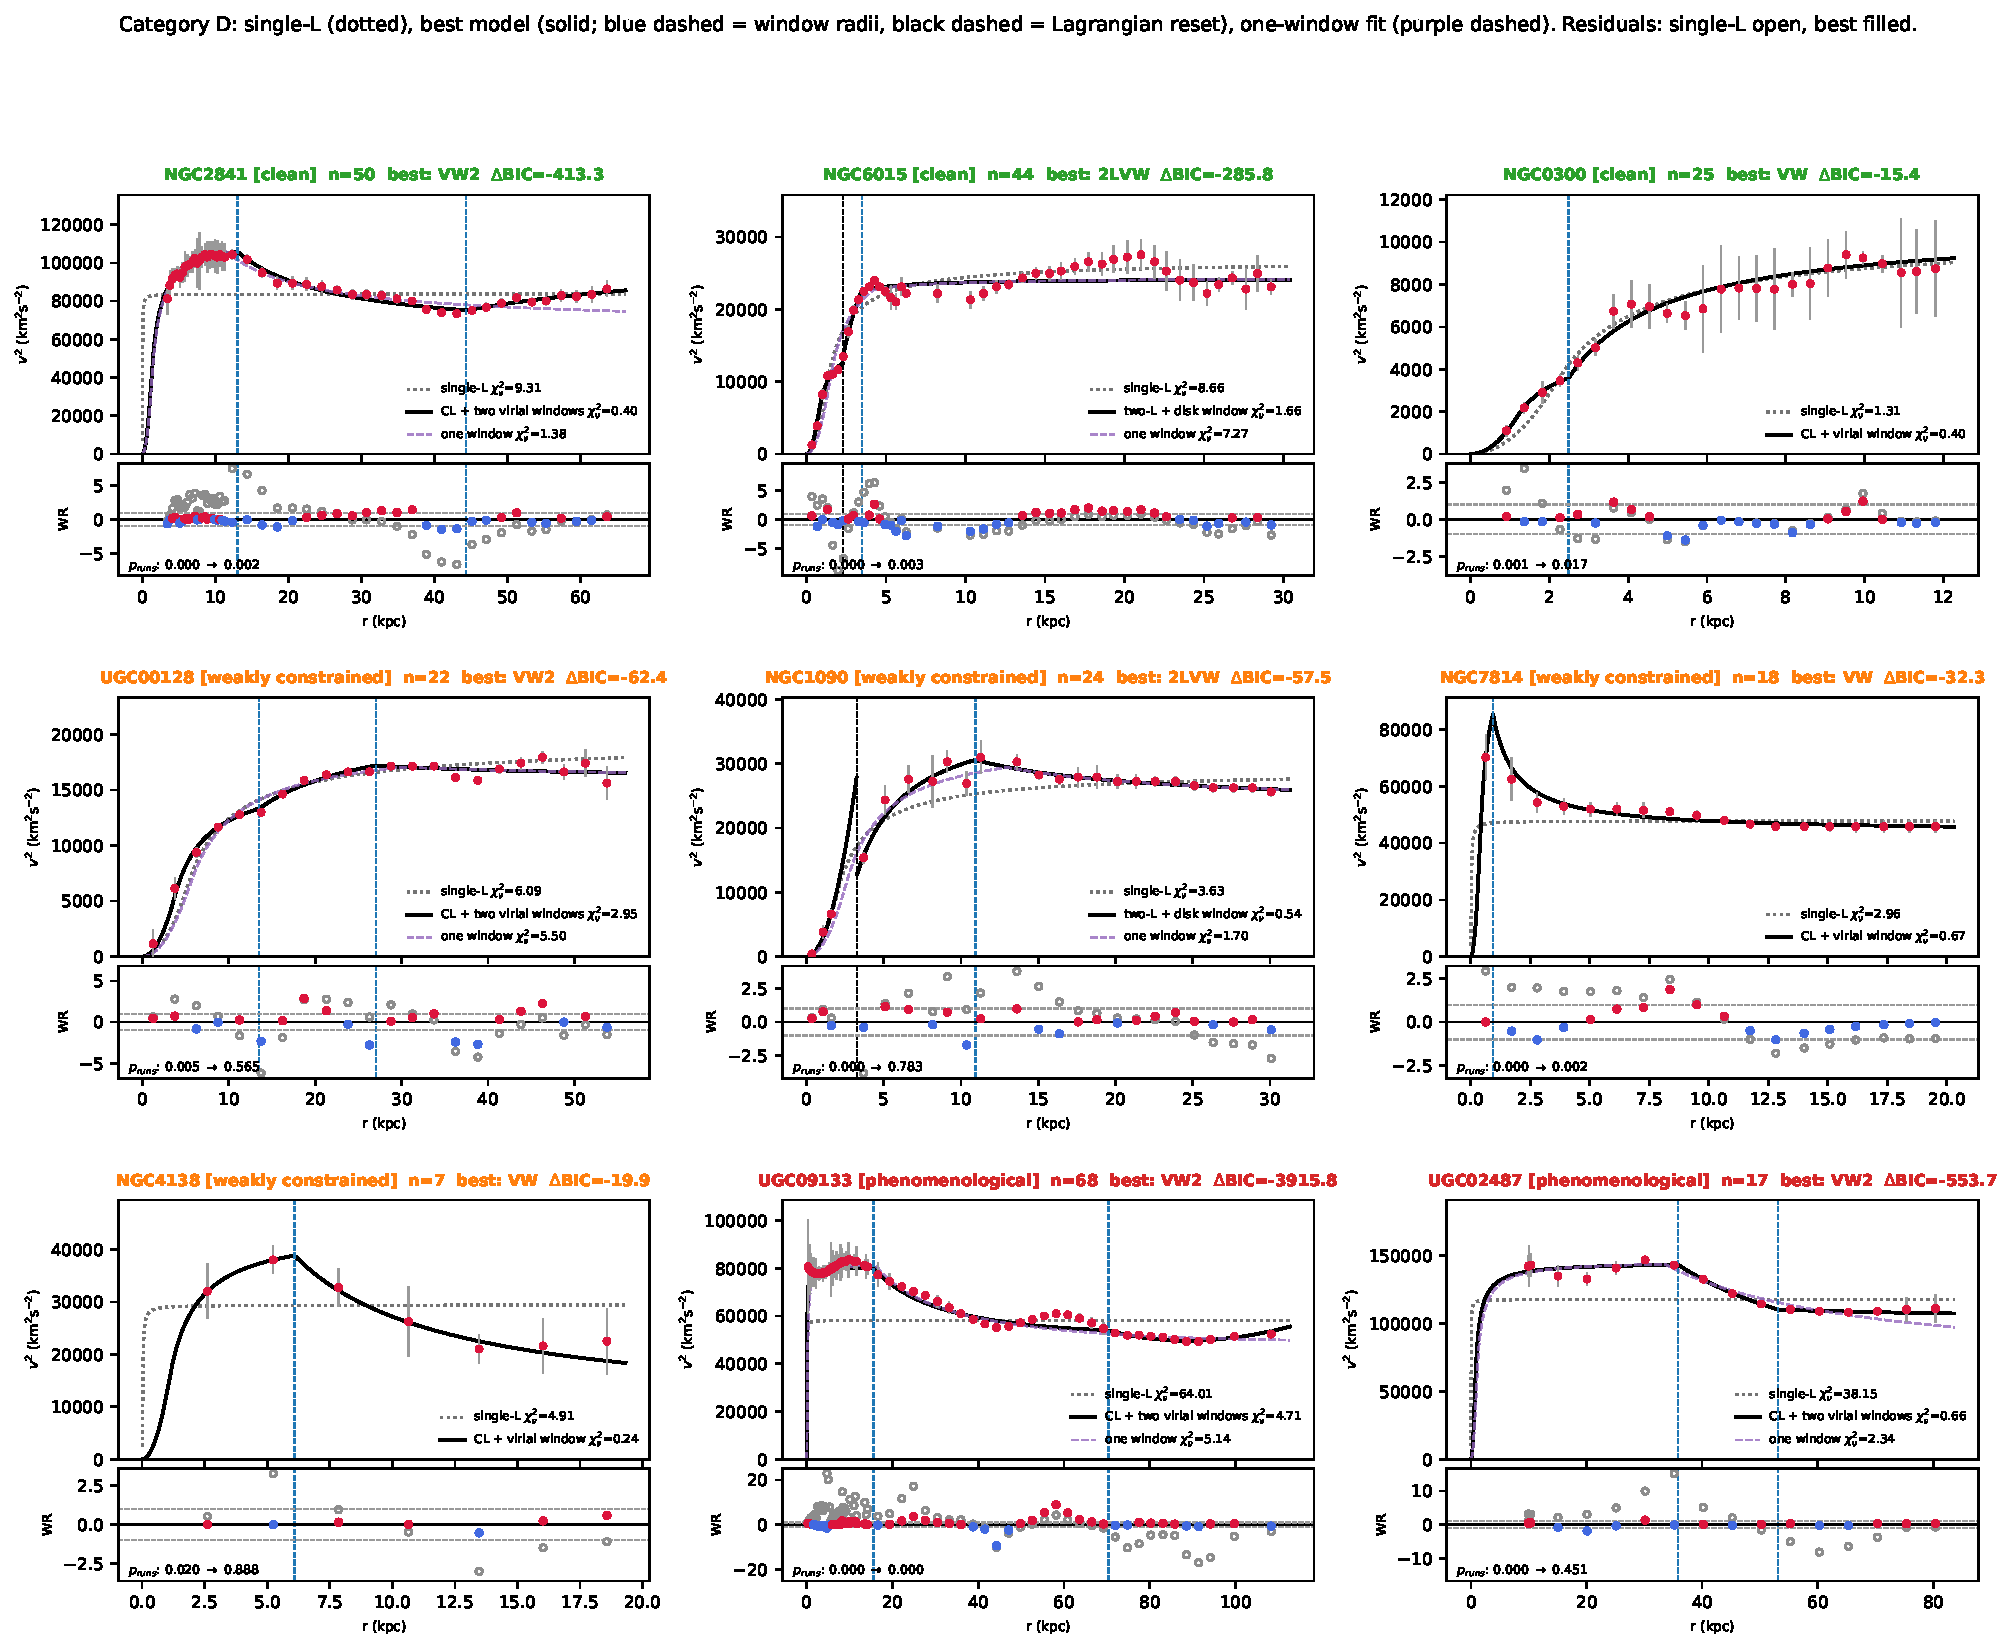
\includepdf[pages=-,landscape=true,scale=0.95]{catD_atlas.pdf}\end{document}